\documentclass{beamer}
\usepackage{comment}
\usepackage[english]{babel}
\usepackage[utf8]{inputenc}
\usepackage{amsmath, amssymb, amsthm}
\usepackage{cmap}
\usepackage[T1]{fontenc}
\usepackage{array}
\usepackage{multicol}
\usepackage{multirow}
\usepackage{blindtext}
\usepackage{subcaption}
\usepackage{bibentry}
\usepackage{wasysym}
\usepackage{makecell}
\usepackage{marvosym}
%\usepackage{enumitem}
%\definecolor{UBCblue}{rgb}{0.09412, 0.27450, 0.53334}
\definecolor{FMFI}{rgb}{1, 0.5098, 0}
\usetheme{default}
\useinnertheme{circles}
\usecolortheme[named=FMFI]{structure}
\setbeamercolor{block body}{bg=FMFI!10}
\setbeamercolor{block title}{bg=FMFI!30}
\setbeamertemplate{blocks}[rounded][shadow]
\setbeamertemplate{navigation symbols}{}
\setbeamertemplate{itemize item}[default]
\usepackage{tikz}
\usetikzlibrary{shapes.geometric}
\usefonttheme[onlymath]{serif}
% \usetikzlibrary{external}
% \tikzexternalize[prefix=images/]
\newtheorem{conjecture}{Conjecture}
\newtheorem{proposition}{Proposition}
\setbeamertemplate{footline}[frame number]
\usepackage{cite}
\renewcommand*{\citeleft}{\!\!}
\renewcommand*{\citeright}{}
% -------------------
% --- Definicia zakladnych pojmov
% --- Vyplnte podla vasho zadania, rok ma byt rok odovzdania
% -------------------
\def\mfrok{2026}
\def\mfnazov{New approaches to nowhere-zero flow problems}
\def\mftyp{Diploma Thesis}
\def\mfautor{Bc. Lukáš Gáborik}
\def\mfskolitel{Mgr. Jozef Rajník, PhD.}
\def\mfoponent{...}

%ak mate konzultanta, odkomentujte aj jeho meno na titulnom liste
\def\mfkonzultant{tit. Meno Priezvisko, tit. }  

\def\mfmiesto{Bratislava, \mfrok}

% študenti BIN a DAV odkomentujú príslušnú dvojicu riadkov
\def\mfodbor{Computer Science}
\def\program{Computer Science }
% pre BIN:
%\def\mfodbor{Computer Science and Biology} 
%\def\program{ Bioinformatics }
% pre DAV:
% \def\mfodbor{Computer Science and Mathematics} 
% \def\program{Data Science}

% Ak je školiteľ z FMFI, uvádzate katedru školiteľa, zrejme by mala byť aj na zadaní z AIS2
% Ak máte externého školiteľa, uvádzajte Katedru informatiky 
\def\mfpracovisko{Department of Computer Science}


\title{\mfnazov}

\subtitle{Master thesis}

\author
{Lukáš Gáborik}

\institute[]
{
  \begin{figure}
      \centering
      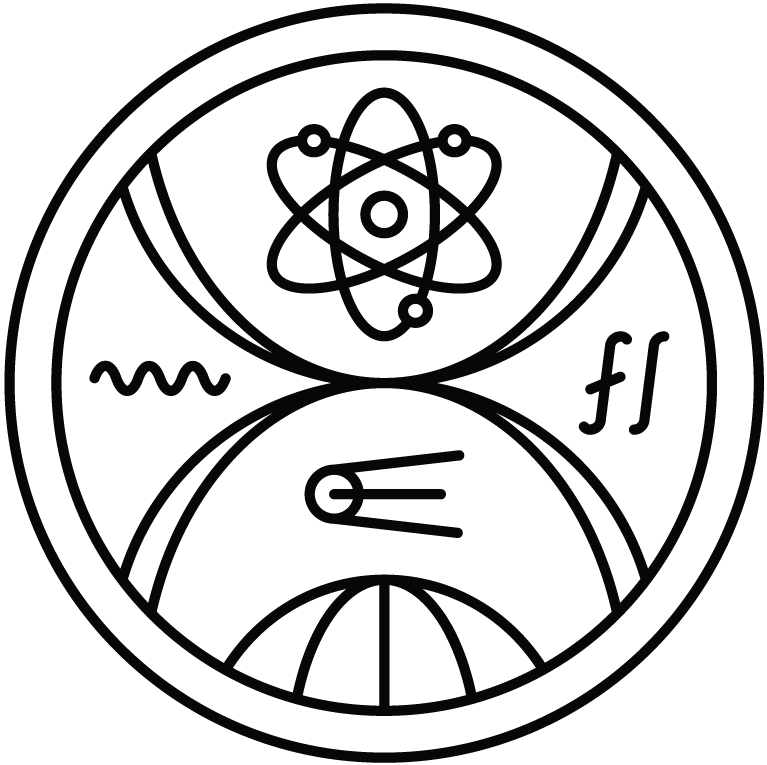
\includegraphics[width=0.15\linewidth]{../logo_FMFI.png}
  \end{figure}
}

\date{21$^\text{st}$ January 2025}

\AtBeginSection[]

\begin{document}

\begin{frame}\titlepage\end{frame}

\begin{frame}{Nowhere-zero $k$-flows}
	\begin{figure}
		\centering
		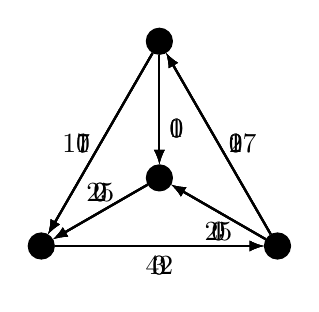
\begin{tikzpicture}[auto,scale=0.5]

	\node (c0) [circle, draw, fill=black] at (0, 0) {};
	\node (c1) [circle, draw, fill=black] at (6, 0) {};
	\node (c2) [circle, draw, fill=black] at (3, 5.2) {};
	\node (c3) [circle, draw, fill=black] at (3, 1.73) {};

	\path<1>
	(c0) edge[-latex, thick] node[below] {$42$} (c1)
	(c1) edge[-latex, thick] node[right] {$17$} (c2)
	(c2) edge[-latex, thick] node[below right] {$0$} (c3)
	(c2) edge[-latex, thick] node[left] {$17$} (c0)
	(c3) edge[-latex, thick] node[above] {$25$} (c0)
	(c1) edge[-latex, thick] node[below] {$25$} (c3);
	
	\path<2>
	(c0) edge[-latex, thick] node[below] {$0$} (c1)
	(c1) edge[-latex, thick] node[right] {$0$} (c2)
	(c2) edge[-latex, thick] node[below right] {$0$} (c3)
	(c2) edge[-latex, thick] node[left] {$0$} (c0)
	(c3) edge[-latex, thick] node[above] {$0$} (c0)
	(c1) edge[-latex, thick] node[below] {$0$} (c3);
	
	\path<3>
	(c0) edge[-latex, thick] node[below] {$3$} (c1)
	(c1) edge[-latex, thick] node[right] {$2$} (c2)
	(c2) edge[-latex, thick] node[below right] {$1$} (c3)
	(c2) edge[-latex, thick] node[left] {$1$} (c0)
	(c3) edge[-latex, thick] node[above] {$2$} (c0)
	(c1) edge[-latex, thick] node[below] {$1$} (c3);

\end{tikzpicture}

		\caption{\only<1>{$43$-flow}\only<2>{$1$-flow}\only<3>{NZ $4$-flow, $\Phi(K_4)=4$}}
	\end{figure}
	\begin{itemize}
		\item<1-> assignment of values $0, 1, 2, \dots, k-1$ to edges
		\item<1-> Kirchoff's law in vertices
		\item<2-> this allowing trivial cases
		\item<2-> restrict zero flow values
		\item<3> graph with NZ $k$-flow has also a NZ $(k+1)$-flow
		\item<3> rate of graph complexity
		\item<3> flow number $\Phi(\Gamma)$ -- minimum
	\end{itemize}
\end{frame}

\end{document}
